%\documentclass[theoremcontinuousnumbering,notnumberedtheorems]{actacybpress}
%\documentclass[theoremsectionnumbering,notnumberedtheorems]{actacybpress}
\documentclass[notnumberedtheorems,withtitlethanks]{actacyb}
%\documentclass{actacybpress}

% Provides line numbers for the referee.
%\referee

% Draws the border of textbox.
%\usepackage{showframe}

\usepackage{graphicx, algorithm, algorithmic}
% Please use only packages that are absolutely necessary!
% Avoid modifying the page size and layout!

% Class file actacyb.cls requires the hyperref package.
% Here we define metadata and colors used by hyperref.
\hypersetup{
    unicode=true,            % non-Latin characters in Acrobat’s bookmarks
    pdftitle={Title},        % title
    pdfauthor={Authors},     % author
    pdfsubject={Manuscript submitted to Acta Cybernetica},   % subject of the document
    colorlinks=true,         % false: boxed links; true: colored links
    linkcolor=blue,          % color of internal links (change box color with linkbordercolor)
    citecolor=blue,          % color of links to bibliography
    filecolor=blue,          % color of file links
    urlcolor=blue            % color of external links
}

\begin{document}

% Overfull boxes can be avoided by using the \sloppy command.
% Use it as a last chance only since it produces underfull boxes.
% \fussy resets to the normal setting.
%\sloppy
%...
%\fussy

%% Uncomment commands below once the required information is known
%% Used by the technical editor
%\acta{vol}{num}{year}{paper_id}
%\setcounter{page}{1}
%\received{...} 

\title{The Title of the Article\thanks{This work was supported by... If such a thanks text is included, use the {\tt withtitlethanks} option of the {\tt actacyb} document class!}}
%\headingtitle{If title gets too long put a shorter version here}

\author{
First Author\thanks{Affiliation of first and second author} \thanks{\email{firstauth@email.address}, \orcid{xxxx-xxxx-xxxx-xxxx}} , Second Author\thanksmark{2} \thanks{\email{secondauth@email.address}, \orcid{xxxx-xxxx-xxxx-xxxx}} ,
\and Third Author\thanks{Affiliation of third author} \thanks{\email{thirdauth@email.adress}, \orcid{https://orcid.org/xxxx-xxxx-xxxx-xxxx}}}
\headingauthor{First Author, Second Author, and Third Author}

% Please provide ORCIDs for all authors!

\maketitle


\begin{abstract}
Here comes the abstract of the article, which is a summary of the main results discussed in the article. It should contain neither mathematical formulas, nor references. 

\keywords{computer science, \LaTeX, article format}
\end{abstract}


\section{Introduction}

The paper should be written in standard \LaTeX using the provided \verb|actacyb.cls| class file. Please do not use strange formats or non-standard packages. Avoid commands that would reconfigure the size of the page, the size and type of letters or the baselineskip. 

The article in the first phase should be written including the \verb|\showframe| package that makes the overfull boxes visible. Before sending the final version of your manuscript, please be sure that there are no such overfull boxes.


\section{Pictures and figures}
Every figure should appear in the \texttt{figure} environment, i.e.\ must be defined between \verb|\begin{figure}| and \verb|\end{figure}|. You should provide where you prefer to put your figure \verb|[htbp]| (h -- here, t -- top, b -- bottom, p -- page), e.g., \verb|\begin{figure}[!ht]| (insert figure here or top of next page if does not fit).

Primarily we use \verb|pdflatex| to generate a PDF result of your document.
As such, preferably include images in Portable Network Graphics (PNG) or Portable Document Format (PDF) formats with the e.g., \verb|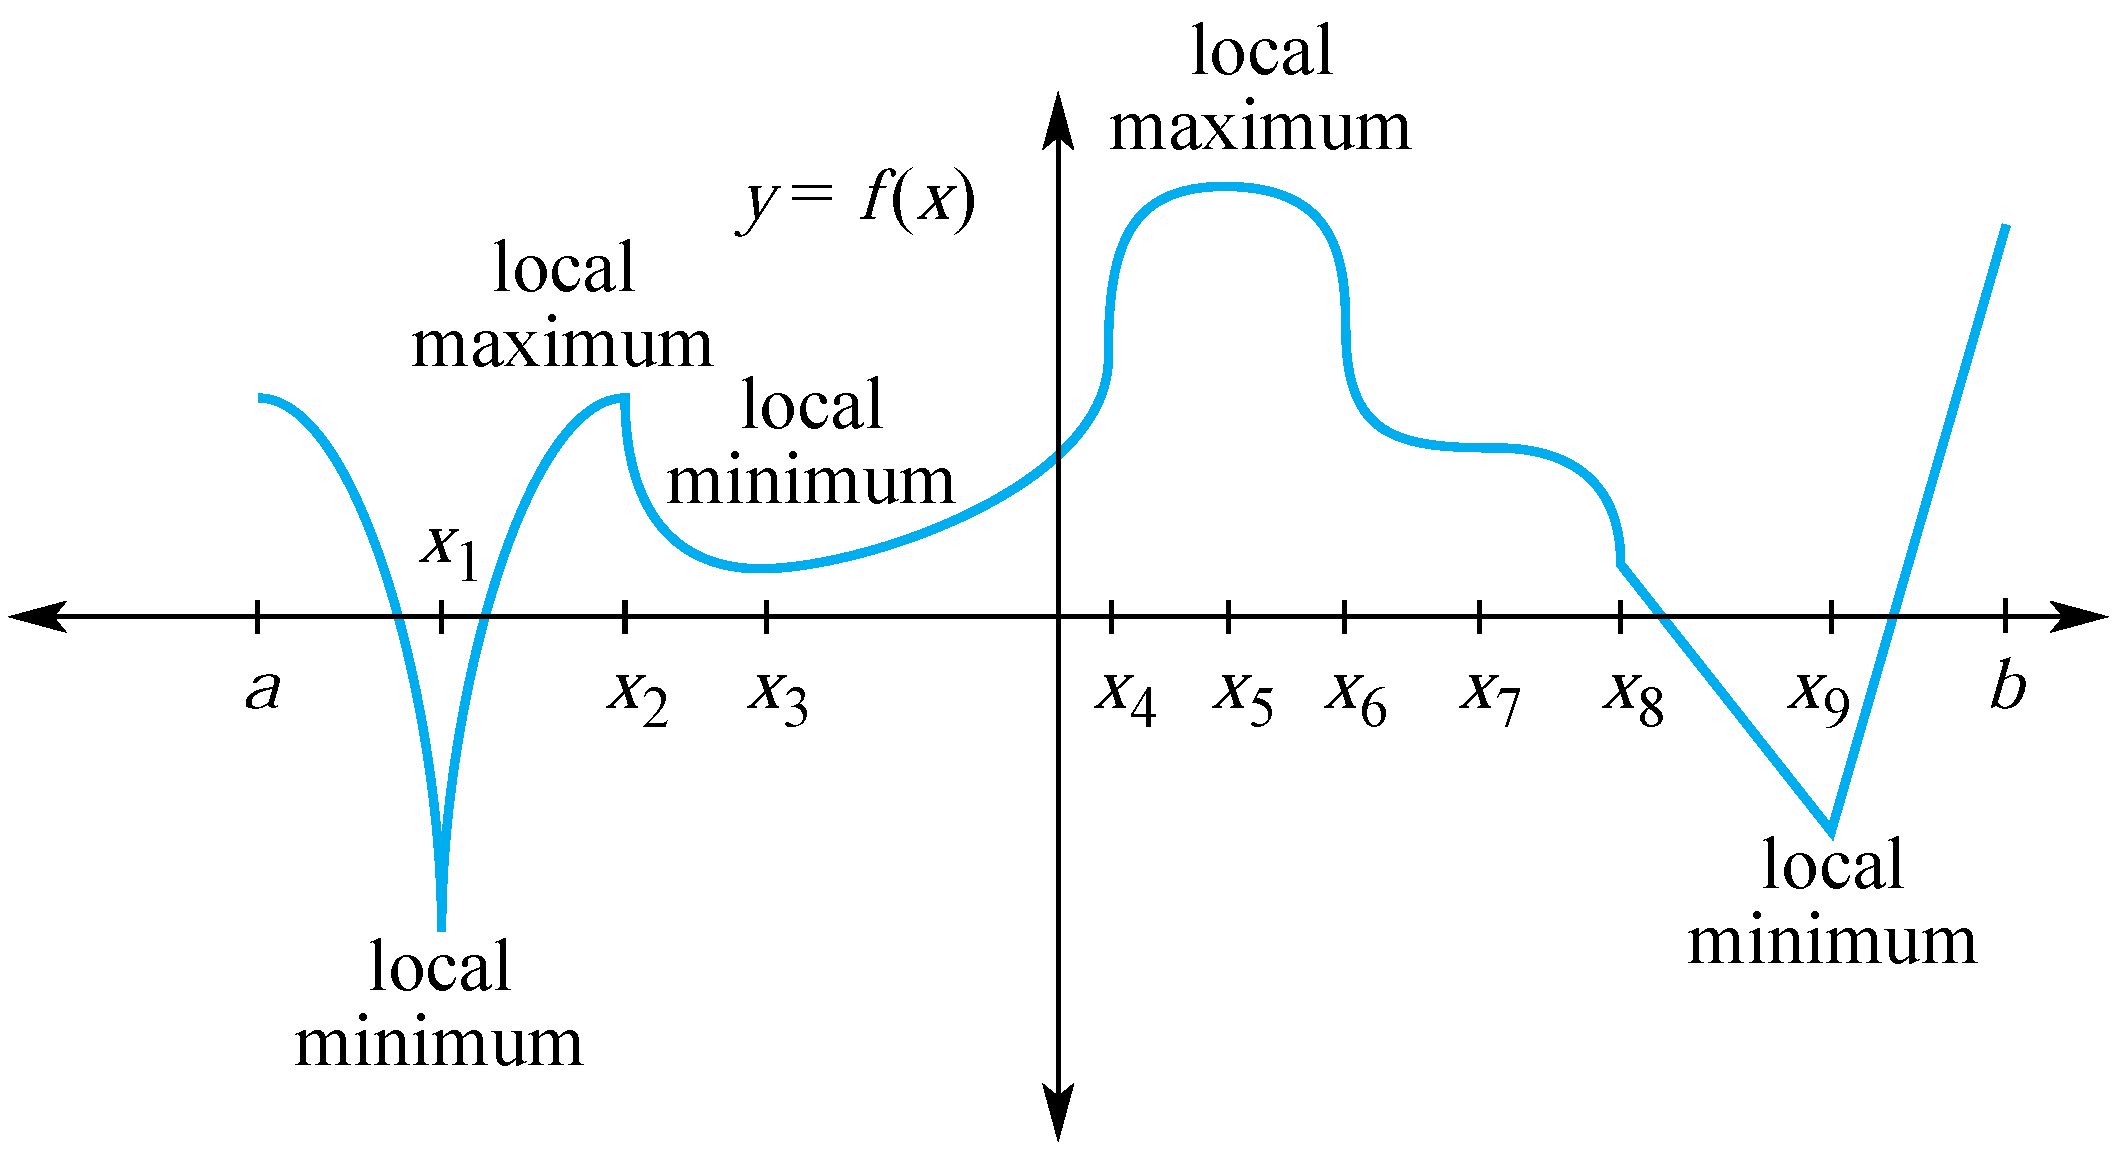
\includegraphics{example.png}| command. 
Alternatively \LaTeX\ figures, PostScript(.ps) or Encapsulated PostScript (.eps) images can also be used with \verb|latex| used for compiling.

Using drawing packages such as {\verb|tikz|} or calling shell executables such as \linebreak {\verb|pygmentize|} may cause incompatibilities. If possible, try to generate a separate PDF file of these figures and include this PDF in the manuscript.

Before \verb|\end{figure}| give a title to your figure within the \verb|\caption{...}| command. To be able to refer to this figure later, label it with a unique identifier using the  \verb|\label{uniquelabel}| command. In the text you can refer to it with \verb|\ref{uniquelabel}|. Let us consider the following example:

\begin{verbatim}
Figure \ref{fig:example} shows an example.
\begin{figure}[ht]
\begin{center}
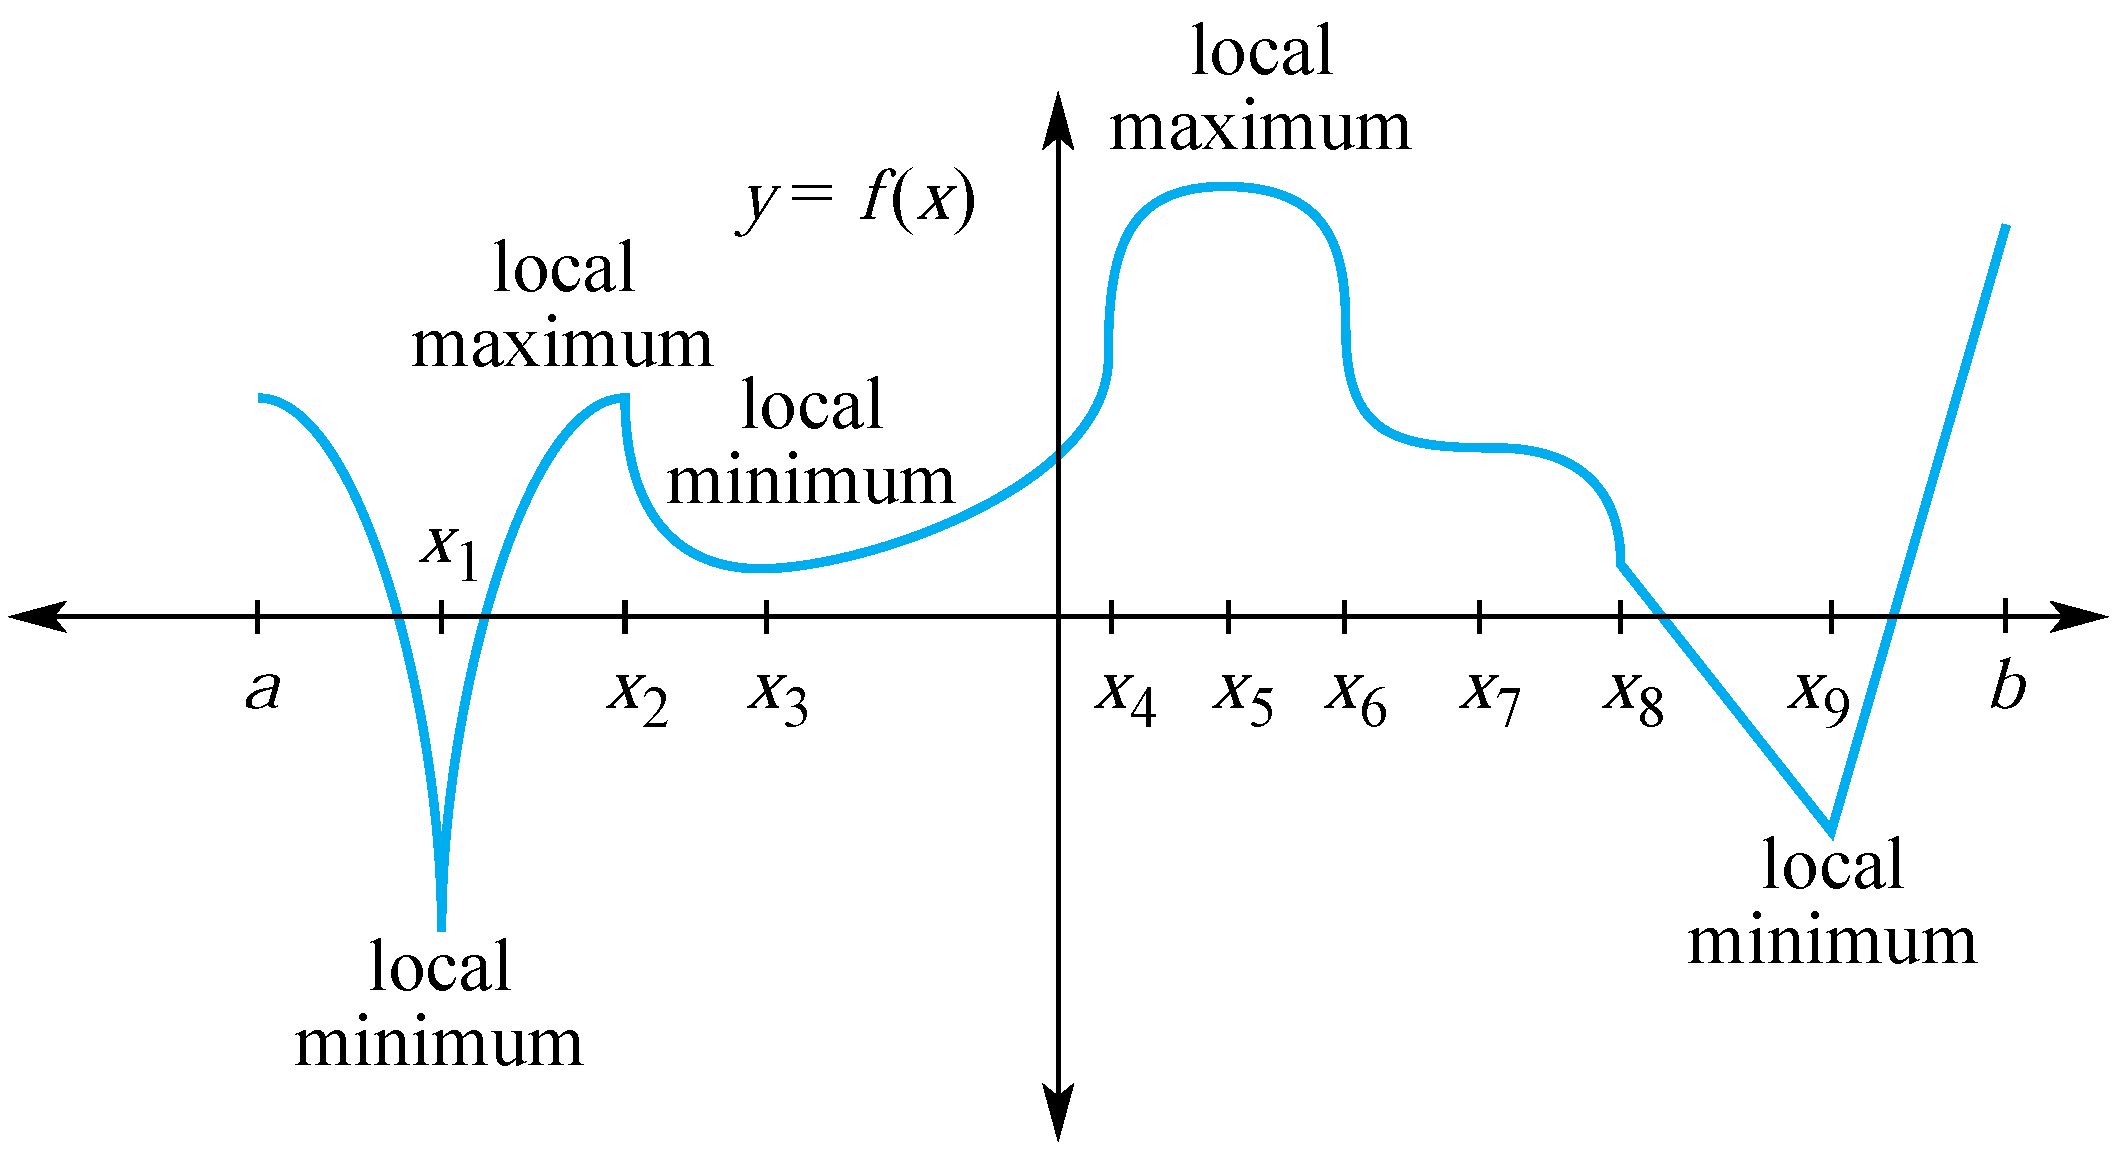
\includegraphics[scale=1.0]{example.png}
\end{center}
\caption{The example figure\label{fig:example}}
\end{figure}
\end{verbatim}

Figure \ref{fig:example} shows an example.
\begin{figure}[ht]
\begin{center}
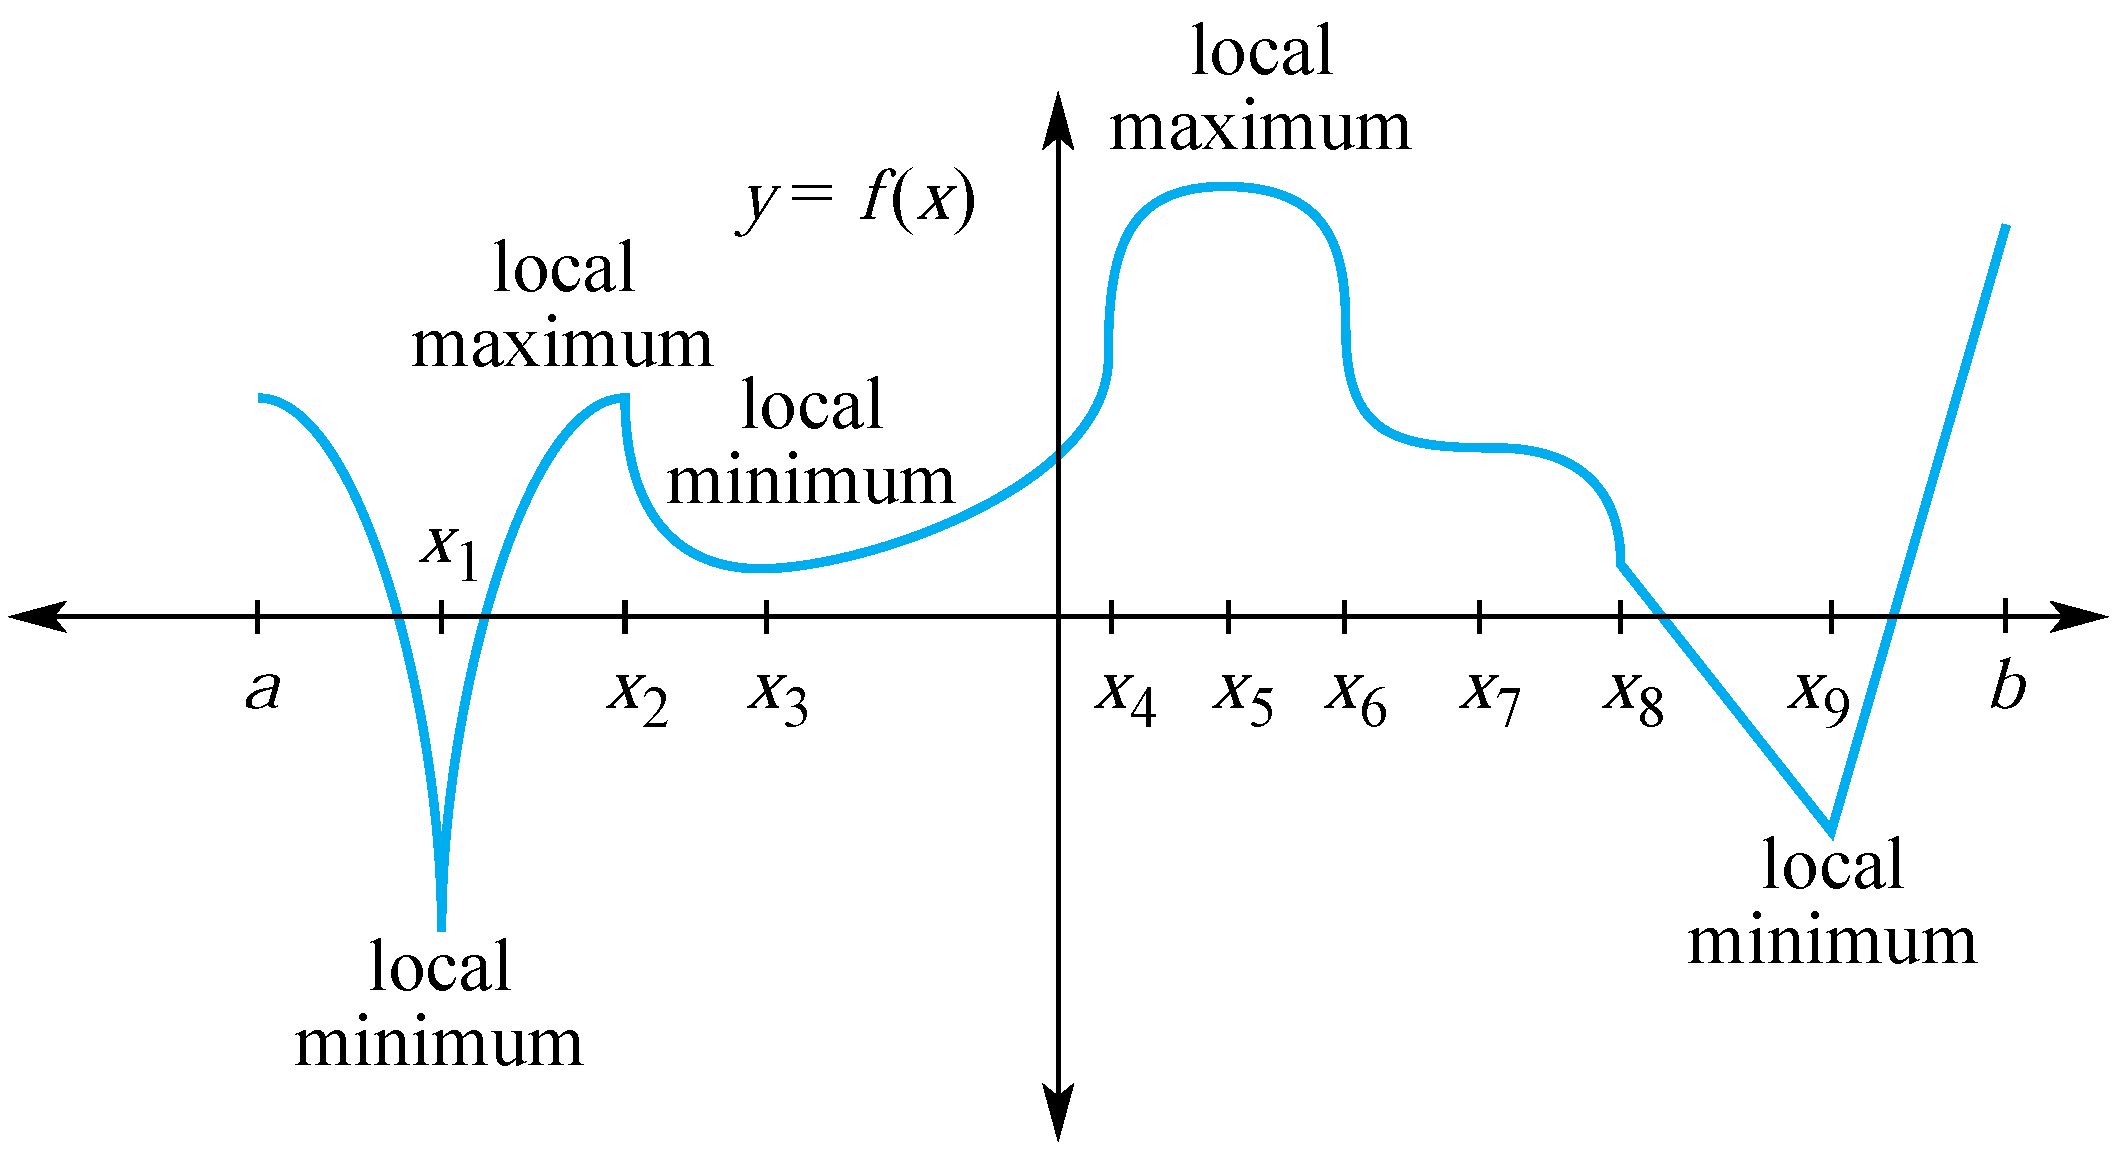
\includegraphics[scale=1.0]{example.png}
\end{center}
\caption{The example figure\label{fig:example}}
\end{figure}


\section{Tables}

Similarly to the procedure with figures, use the \verb|table| environment to create tables.
Normally, the title appears above the table, therefore put the \verb|\caption{...}| command right after \verb|\begin{table}[htbp]|. Use the \verb|tabular| environment to prepare your table.

\begin{verbatim}
\begin{table}[ht]
\caption{This is an example table.}\label{tab:res}
\begin{center}
\begin{tabular}{l|rr}
Problem & Time(s) & Memory(MB) \\ \hline
easy    & 13   & 25   \\
hard    & 2359 & 6820 \\
\end{tabular}
\end{center}
\end{table}
Table \ref{tab:res} shows an example table.
\end{verbatim}

\begin{table}[ht]
\caption{This is an example table.}\label{tab:res}
\begin{center}
\begin{tabular}{l|rr}
Problem & Time(s) & Memory(MB) \\ \hline
easy    & 13   & 25   \\
hard    & 2359 & 6820 \\
\end{tabular}
\end{center}
\end{table}
Table \ref{tab:res} shows an example table.


\section{Theorems and Lemmas}

In the \verb|actacyb| class the \verb|amsthm| package is included.
Thus, the most common environments, such as \verb|definition|, \verb|theorem|, \verb|lemma|,
\verb|proposition|, \verb|corollary|, \verb|claim|, \verb|remark|, \verb|example| and \verb|proof| are already defined.
To define other environments, please use the \verb|\newtheorem{otherenv}[theorem]{Otherenv}|  
command.

Please do not redefine the theoremstyle or theorem numbering. 
By default, each ``theorem'' type is consecutively numbered:
\texttt{Theorem 1}, \texttt{Theorem 2}, \texttt{Lemma 1}, etc.
throughout the paper.
If you need numbering by sections, you should indicate it as an option to
\verb|\documentclass| at the beginning of the document:

\begin{verbatim}
\documentclass[theoremsectionnumbering]{actacyb.cls}
\end{verbatim}

Not numbered theorem environments can also be used by specifying the option \verb|notnumberedtheorems| for \verb|documentclass|. Such environment names have an ``nn'' prefix, e.g., \verb|nntheorem|, \verb|nndefinition|, \verb|nnremark|.
If you would like to specify the default numbering behaviour explicitly, use the
\verb|theoremcontinuousnumbering| option.

The \verb|proof| environment automatically generates the end of proof (qed) symbol
at the end of the proof. If you don't need this symbol, redefine it to an empty command
inside the proof environment (for the given proof only) or in the preamble (globally) as \verb|\renewcommand{\qedsymbol}{}|.

By using the \verb|theoremcontinuousnumbering| and \verb|notnumberedtheorems| options, the following commands produce the result below:

\begin{verbatim}
\begin{definition}
We define....
\end{definition}

\begin{theorem}
If $N=1$, then $P=NP$.
\end{theorem}

\begin{proof}
It is easy to see that if $N=1$, then $NP=1\cdot P = P$.
\end{proof}

\begin{nnremark}
This is a not numbered remark.
\end{nnremark}

\begin{definition}
We define....
\end{definition}

\begin{remark}
Let us note that the above theorem is not...
\end{remark}
\end{verbatim}


\begin{definition}
We define....
\end{definition}

\begin{theorem}
If $N=1$, then $P=NP$.
\end{theorem}

\begin{proof}
It is easy to see that if $N=1$, then $NP=1\cdot P = P$.
\end{proof}

\begin{nnremark}
This is a not numbered remark.
\end{nnremark}

\begin{definition}
We define....
\end{definition}

\begin{remark}
Let us note that the above theorem is not...
\end{remark}

By specifying the {\tt theoremsectionnumbering} option at the \verb|documentclass|
declaration, we would see \textbf{Definition 4.1}, \textbf{Theorem 4.1}, \textbf{Remark}, and \textbf{Remark 4.1} captions here, respectively.


\section{Equations}

The usual way to write equations is to use the \verb|equation| environment for a single line
of equation, and the \verb|eqnarray| environment for multiline equations.
It is also possible to use the \verb|array| environment within an \verb|equation|,
but we do not recommend its usage, because its spacing and labeling may not give the desired result.
Besides the \verb|equation| and \verb|eqnarray| environments,
other \verb|amstex| environments, such as \verb|multiline|, \verb|align|, \verb|split|, etc. 
are also recommended.

\begin{verbatim}
The function $\Phi$ is defined in formula \ref{eq:phi}.

\begin{equation}
\Phi(x)=\prod_{i=1}^n\sin(x_i)\cos(x_i-\frac{1}{3}\pi)\label{eq:phi}
\end{equation}
\end{verbatim}

The function $\Phi$ is defined in formula (\ref{eq:phi}).

\begin{equation}
\Phi(x)=\prod_{i=1}^n\sin(x_i)\cos(x_i-\frac{1}{3}\pi)\label{eq:phi}
\end{equation}


\section{Indentations}

Below is an example of text indentation:

\begin{verbatim}
In addition, seeds have the following property:

\begin{itemize}
\item[] 
If a seed of clause $c_T$, and example {\bf x} satisfies 
$c_T$ but not $c$, then {\bf x} has at least one attribute 
in $c_T$ that is not in $c$.\hfill({\tt*})
\end{itemize}
The procedure below...
\end{verbatim}

In addition, seeds have the following property:

\begin{itemize}
\item[] 
If a seed of clause $c_T$, and example {\bf x} satisfies $c_T$ but
not $c$, then {\bf x} has at least one attribute in $c_T$ that
is not in $c$.\hfill({\tt*})
\end{itemize}
The procedure below...

\subsection{Bulleted List}

Below is an example of a bulleted list:

\begin{verbatim}
\begin{itemize}
\item for every $x\in A$ and for...
\item for every $x_1$, $x_2$ and for every...
\end{itemize} 
\end{verbatim}

\begin{itemize}
\item for every $x\in A$ and for...
\item for every $x_1$, $x_2$ and for every...
\end{itemize} 

\subsection{Enumerated List}
Below is an example of an enumerated list:

\begin{verbatim}
\begin{enumerate}
\item If one of the following conditions holds:
\begin{enumerate}
\item The first condition.\label{step:1a}
\item The second condition.
\end{enumerate}
\item If ${n\over n_1}=3$ then in the majority of cases the 
assumption may be removed.
\end{enumerate}

Let us refer to the first condition by \ref{step:1a}.
\end{verbatim}

\begin{enumerate}
\item If one of the following conditions holds:
\begin{enumerate}
\item The first condition.\label{step:1a}
\item The second condition.
\end{enumerate}
\item If ${\frac{n}{n_1}}=3$ then in the majority of cases the 
assumption may be removed.
\end{enumerate}

Let us refer to the first condition by \ref{step:1a}.


\section{Algorithms}

If you want to include algorithms in your manuscript, please use the \verb|algorithm| package along with the \verb|algorithmic| style.
As in other floating environments, please use some of the \verb|[htbp]| (h -- here, t -- top, b -- bottom, p -- page) letters right after \verb|\begin{algorithm}| to determine the desired place of your algorithm. Please provide a title with the \verb|\caption{...}| command, and use the \verb|\label{alg:...}| and \verb|\ref{alg:...}| commands if you want to refer to the algorithm in the text, as shown in the following example.
If you have the latest \verb|algorithmic| package, you can also refer to any step of the algorithm as shown in the following example.

\begin{verbatim}
A general Interval Branch and Bound algorithm is shown in 
Algorithm~\ref{alg:ibb}. One of the following selection rules
is applied in Step \ref{step:selrule}:
\begin{algorithm}[ht!]
\caption{ A general interval B\&B algorithm.} 
\label{alg:ibb} 
\textbf{\underline{Funct}} IBB($S,f$)
\renewcommand{\algorithmiccomment}[1]{\hfill {\it #1}}
\begin{algorithmic}[1]
\STATE Set the working list ${\cal L}_W$ := $\{S\}$ and the final 
list ${\cal L}_Q$ := $\{\}$     
\WHILE{( ${\cal L}_W \neq \emptyset$ )} \label{alg:igoend}
  \STATE  Select an interval $X$ from ${\cal L}_W$
                  \label{step:selrule} \COMMENT{Selection rule ~}  
  \STATE Compute $lbf(X)$ \COMMENT{Bounding rule ~}		  
  \IF[Elimination rule]{$X$ cannot be eliminated}
    \STATE Divide $X$ into $X^j,\ j=1,\dots, p$, subintervals   
                                        \COMMENT{Division rule ~}
    \FOR{$j=1,\ldots,p$}
      \IF[Termination rule]{$X^j$ satisfies the termination 
                                                       criterion}
        \STATE Store $X^j$ in ${\cal L}_W$ 
      \ELSE
        \STATE Store $X^j$ in ${\cal L}_W$ 
      \ENDIF
    \ENDFOR  
  \ENDIF
\ENDWHILE
\STATE \textbf{return} ${\cal L}_Q$
\end{algorithmic}
\end{algorithm}
\end{verbatim}


A general Interval Branch and Bound algorithm is shown in Algorithm~\ref{alg:ibb}. One of the following selection rules is applied in Step \ref{step:selrule}.

\begin{algorithm}[ht!]
\caption{ A general interval B\&B algorithm.} 
\label{alg:ibb} 
\textbf{\underline{Funct}} IBB($S,f$)
\renewcommand{\algorithmiccomment}[1]{\hfill {\it #1}}
\begin{algorithmic}[1]
\STATE Set the working list ${\cal L}_W$ := $\{S\}$ and the final list ${\cal L}_Q$ := $\{\}$     
\WHILE{( ${\cal L}_W \neq \emptyset$ )} \label{alg:igoend}
  \STATE  Select an interval $X$ from ${\cal L}_W$ \label{step:selrule}\COMMENT{Selection rule ~}  
  \STATE Compute $lbf(X)$ \COMMENT{Bounding rule ~}		  
  \IF[Elimination rule]{$X$ cannot be eliminated}
    \STATE Divide $X$ into $X^j,\ j=1,\dots, p$, subintervals   \COMMENT{Division rule ~}
    \FOR{$j=1,\ldots,p$}
      \IF[Termination rule]{$X^j$ satisfies the termination criterion}
        \STATE Store $X^j$ in ${\cal L}_W$ 
      \ELSE
        \STATE Store $X^j$ in ${\cal L}_W$ 
      \ENDIF
    \ENDFOR  
  \ENDIF
\ENDWHILE
\STATE \textbf{return} ${\cal L}_Q$
\end{algorithmic}
\end{algorithm}


\section{Bibliography}
For the bibliography, it is mandatory to use \verb|bibtex| to generate the items to achieve a consistent style!
The \verb|actaplain.bst| file defines the style descriptions that can be used like this:

\begin{verbatim}
\bibliographystyle{actaplain}
\bibliography{actabib}
\end{verbatim}

Replace {\tt actabib} with the name of your {\tt .bib} file.
Refer to an article \cite{ratz99nonsmooth}, a book \cite{Klatte1993a}, a technical report \cite{ratz96optimized}, a manual \cite{T3D},
an article in a book \cite{Fuchi1996a}, a chapter in a book \cite{CORR96}, an unpublished paper \cite{jamartin}, a thesis \cite{braune-diss}, a proceedings \cite{griewank-proceedings}, or an article in proceedings \cite{alefeld-survey} using the \verb|\cite| command!

It is necessary to provide detailed description of the referred items.
Make sure that only those items are included in the \verb|bibtex| file that are actually cited from your manuscript!
Please look up and provide the DOI whenever possible! If not available, provide an URL.
\verb|BibTeX| generates clickable DOI and URL links. Check that they work correctly!

{
\bibliographystyle{actaplain}
\bibliography{actabib}
}

\end{document}
